\usepackage[utf8]{inputenc}
\usepackage[T1]{fontenc}
\usepackage[ngerman]{babel}
\usepackage{array}
\usepackage{bookmark}
\usepackage{textpos}
\usepackage{wasysym}
%\usepackage{listliketab}
\usepackage[NewCommands,NewParameters]{ragged2e}
\usepackage{tikz}
\usepackage{eurosym}
\usepackage{textpos}
\usepackage{comment}

\usetheme{junghans}

\def\insertauthorindicator{Wer?}% Default is "Who?"
\def\insertinstituteindicator{Von?}% Default is "From?"
\def\insertdateindicator{Wann?}% Default is "When?"

%\setbeamertemplate{caption}[numbered]

%%neuer Spaltentyp: linksb"undig + Silbentrennung
\newcolumntype{M}[1]{>{\RaggedRight\hspace{0pt}\arraybackslash}p{#1}}

\author{Marius Spix}

\institute[\raisebox{-1ex}{
\includegraphics[height=0.24cm]{images/JW_Kontur}}]{
\includegraphics[scale=0.3]{images/J_60_Schwarz_Reflex_Blue}}
\title{QM-Cockpit}

\addtobeamertemplate{title page}{\vspace{1\baselineskip}\hspace{-9ex}
\includegraphics[scale=.5]{images/Flaticon_SVGFiles/platform11}\vspace{-2\baselineskip}}

%\addtobeamertemplate{frametitle}{}{
%\begin{textblock*}{100mm}(-4.15cm,-.55cm)
%
\includegraphics[scale=.33]{images/Fahne2}\end{textblock*}
%}

\AtBeginSection{\frame{\sectionpage}}
\AtBeginSubsection{\frame{\subsectionpage}}
\newtranslation[to=ngerman]{Section}{Abschnitt}
\newtranslation[to=ngerman]{Subsection}{Unterabschnitt}

\keywords{Abschlusspr"ufung, Fachinformatiker, SAP, Quali"atsmanagement,
Lager, Warenwirtschaft}
\date{\today}

\frenchspacing

\begin{document}

\setcounter{framenumber}{0} 
\begin{frame}
  \maketitle
\end{frame}

\setcounter{figure}{0}

\begin{frame}{"Ubersicht}
  \tableofcontents
\end{frame}

\section{Projektumfeld}

\subsection{Betrieb}
\begin{frame}[<+->]{Junghans Unternehmensgruppe}
			\begin{block}{Fakten}
				\begin{itemize}[<+->]
						\item Versandhandelsgruppe
						\item Hauptsitz in Aachen
						\item ca. 540 Mitarbeiter
						\item vertreten in 7 L"andern
				\end{itemize}
			\end{block}

			\begin{block}{Sortimente}
				\begin{itemize}[<+->]
						\item Junghans Wolle
						\item Pro-Idee
				\end{itemize}
			\end{block}
\end{frame}

\begin{frame}[<+->]{Organisation \& Datenverarbeitung}
			\begin{block}{Die DV}
				\begin{itemize}
						\item 21 Mitarbeiter
						\begin{itemize}
							\item IT-Services
							\item \alert<6>{Anwendungssysteme}
							\item Betriebsorganisation
						\end{itemize}
				\end{itemize}
			\end{block}
			\pause
			\begin{block}{SAP}
				\begin{itemize}[<+->]
						\item Einf"uhrung: Juli 2011
						\item SAP ECC 6.0
						\item SAP NetWeaver BI 7.1
						\item 3-System-Landschaft
				\end{itemize}
			\end{block}
\end{frame}

\subsection{Prozess Wareneingang}
\begin{frame}{Wareneingang}
 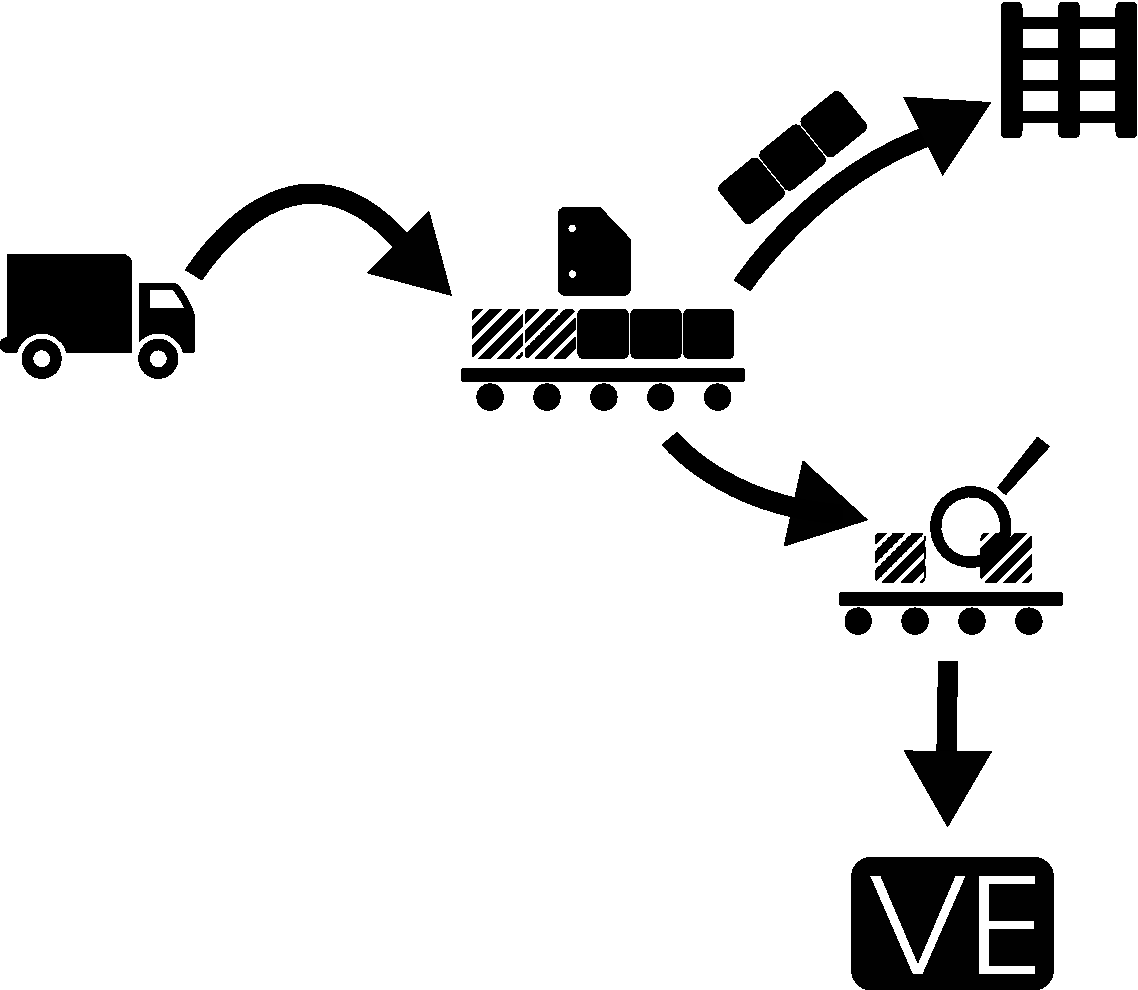
\includegraphics[width=.9\textwidth]{Wareneingang2}
\end{frame}

\section{Das Projekt}
\subsection{Ist-Analyse}
\begin{frame}[<+->]{Analyse}
	\begin{block}{Methoden}
		\begin{itemize}[<+->]
			\item Arbeitsbeobachtung
			\item Interview
			\item Datenbankanalyse
		\end{itemize}
	\end{block}
	\begin{block}{Erkenntnisse}
		\begin{itemize}[<+->]
			\item Personalplanung: saisonale Schwankungen
			\item keine Standardfunktionalit"at
			\item diverse Datenquellen
			\item hoher Normalisierungsgrad
		\end{itemize}
	\end{block}
\end{frame}

\subsection{Soll-Konzept}
\begin{frame}[<+->]{Soll-Konzept}
	\begin{block}{Ziel}
		\begin{itemize}
			\item Vereinfachung der Auswertungen 
			\item zentrale Controlling-Oberfl"ache
			\item Auswertung der Pr"uflosbearbeitungszeit 
		\end{itemize}
	\end{block}
	
	\begin{block}{Kriterien}
		\begin{itemize}
			\item nahtlose Integration in SAP
			\item aktuelle Daten
			\item hohe Performance
			\item Erweiterbarkeit
		\end{itemize}
	\end{block}

\end{frame}

\subsection{Durchf"uhrung}
\begin{frame}{Entwicklungsprozess}
 \includegraphics[width=\textwidth]{FDD}
\end{frame}
\begin{frame}{Aufbau}
 \vspace{3ex}
 \begin{overlayarea}{\textwidth}{\textheight}
  \only<1>{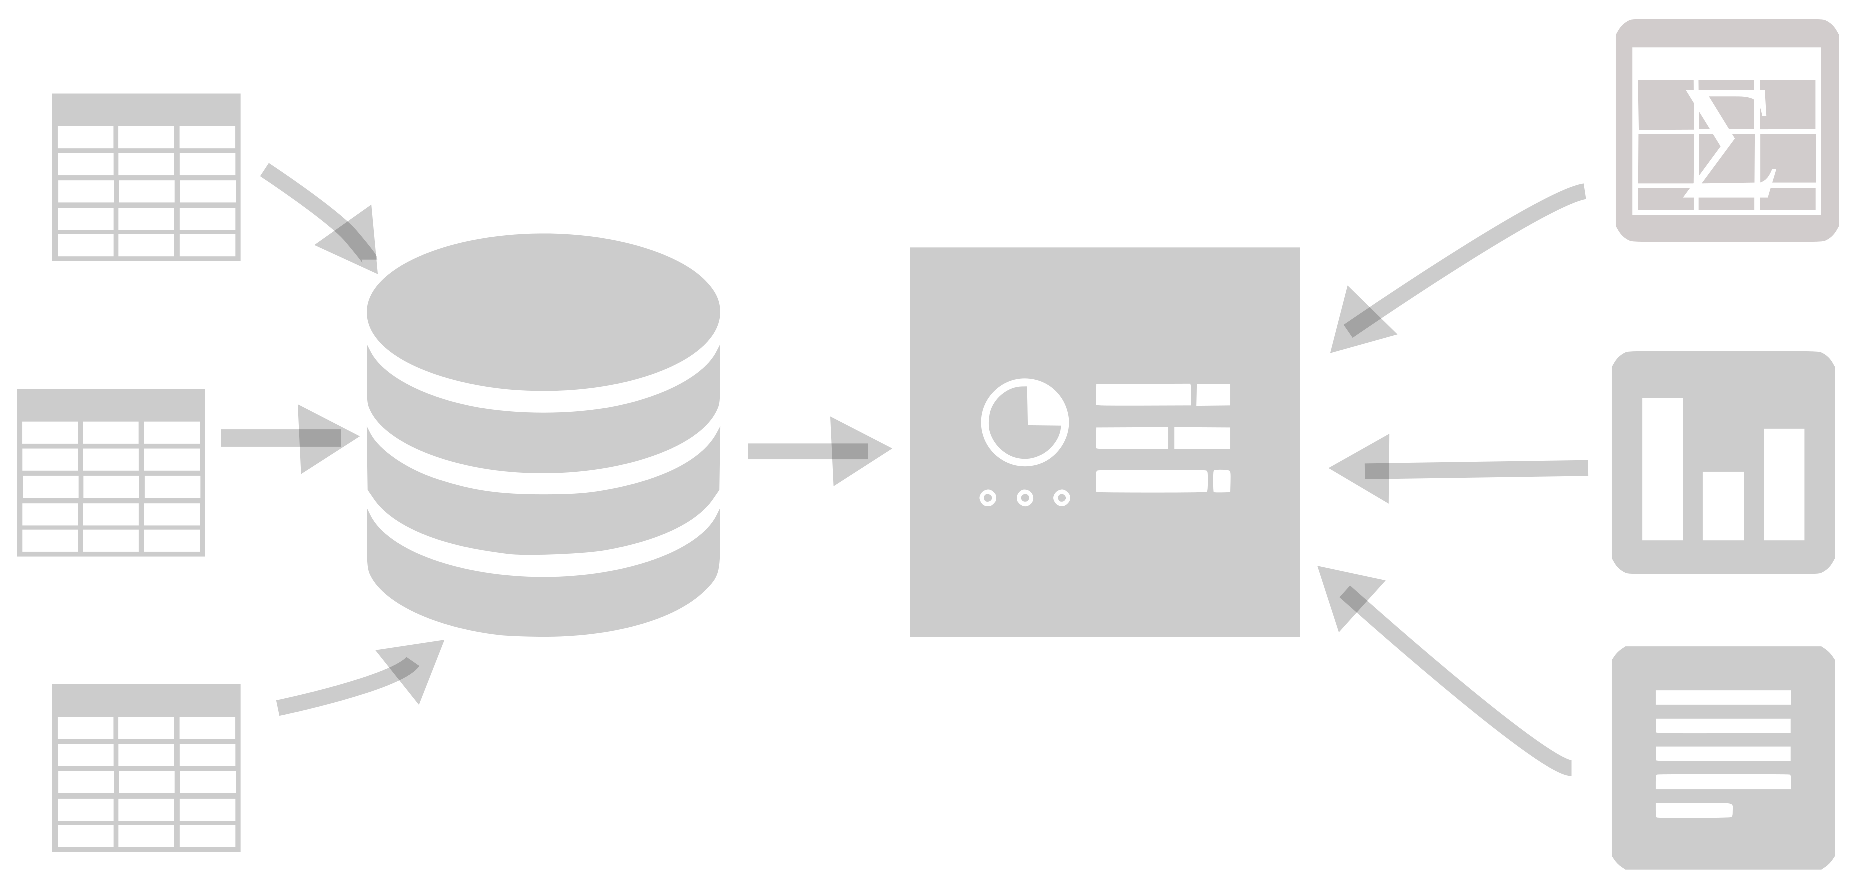
\includegraphics[width=\textwidth]{MVP0}<handout:0>}
  \only<2>{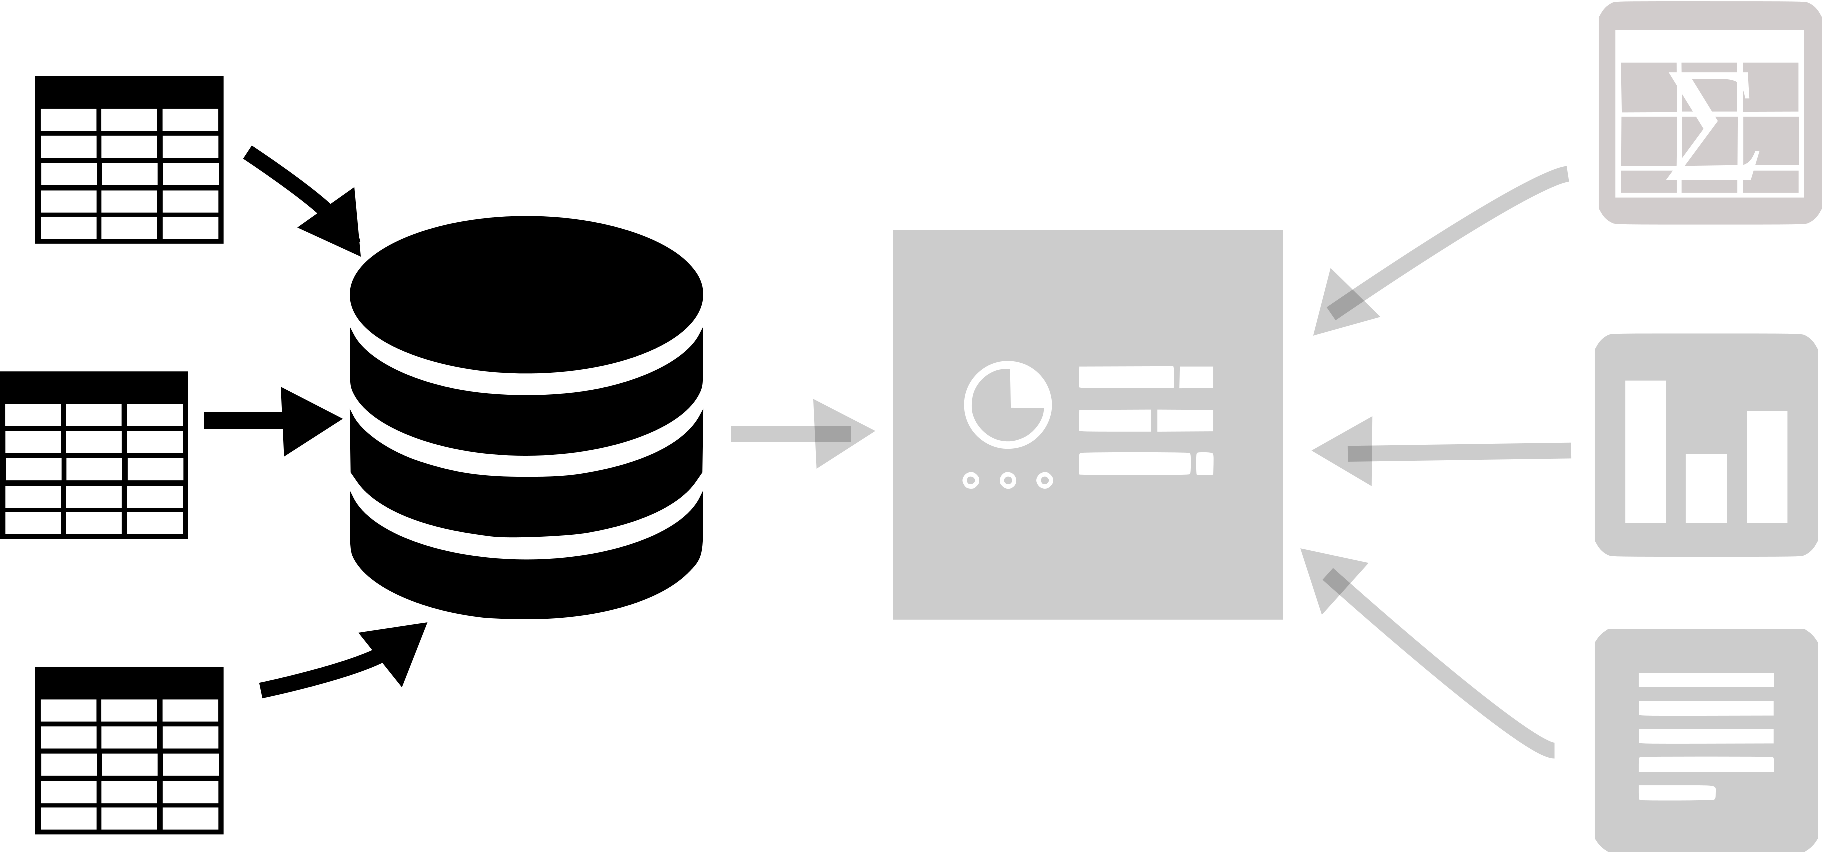
\includegraphics[width=\textwidth]{MVP1}<handout:0>}
  \only<3>{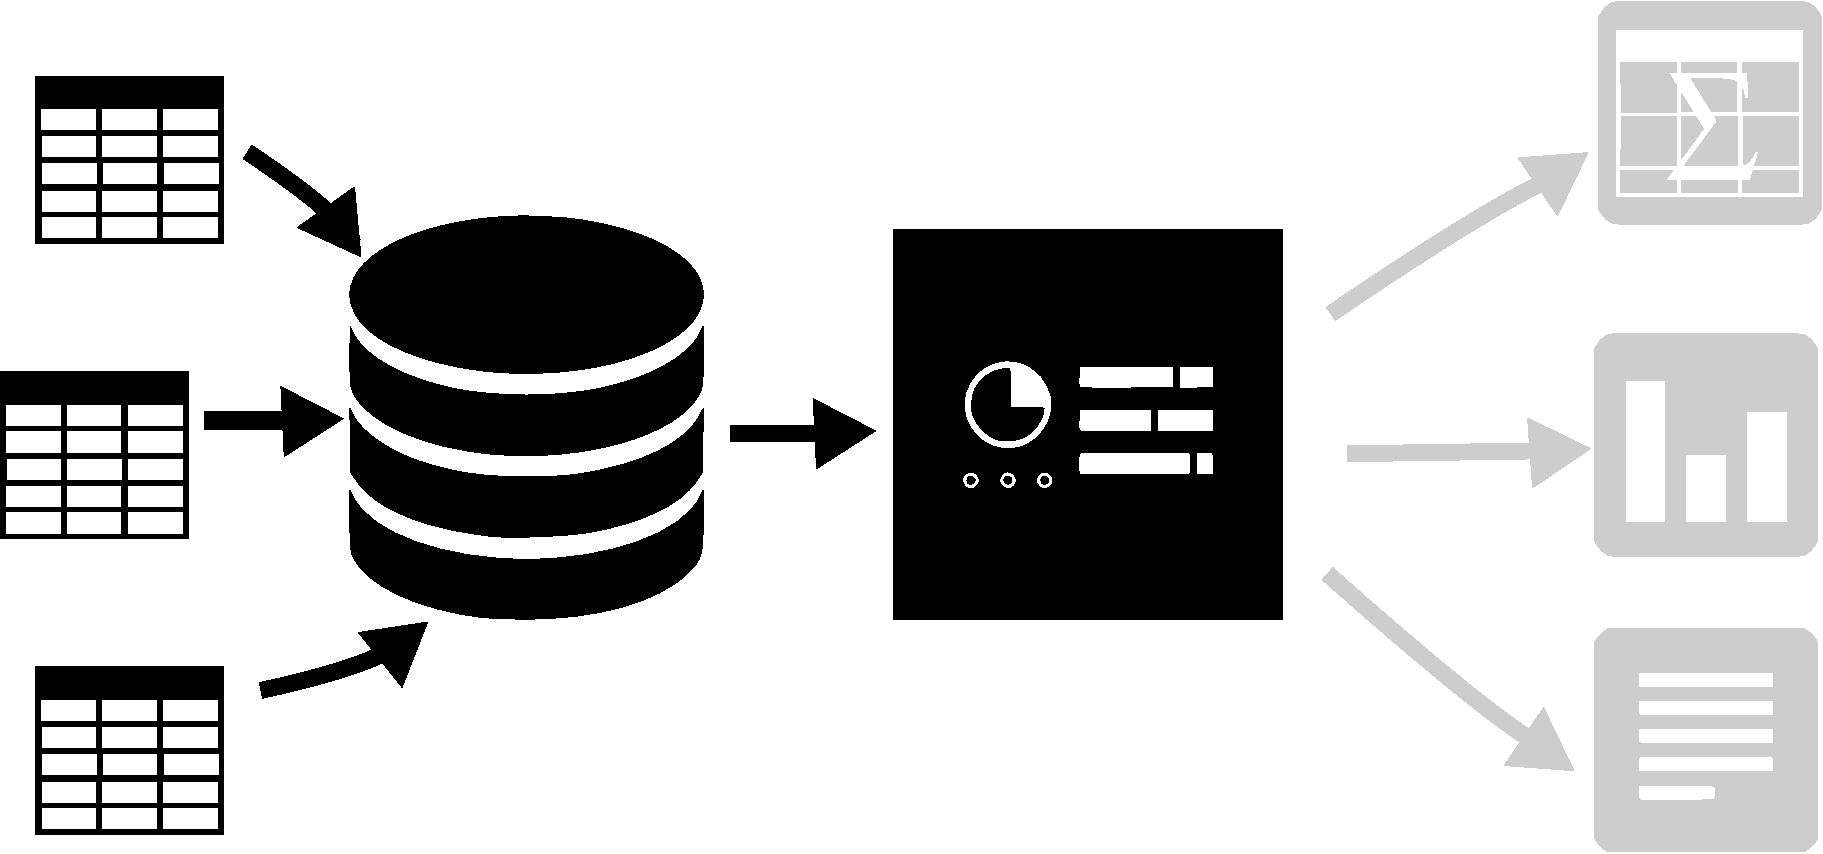
\includegraphics[width=\textwidth]{MVP2}<handout:0>}
  \only<4>{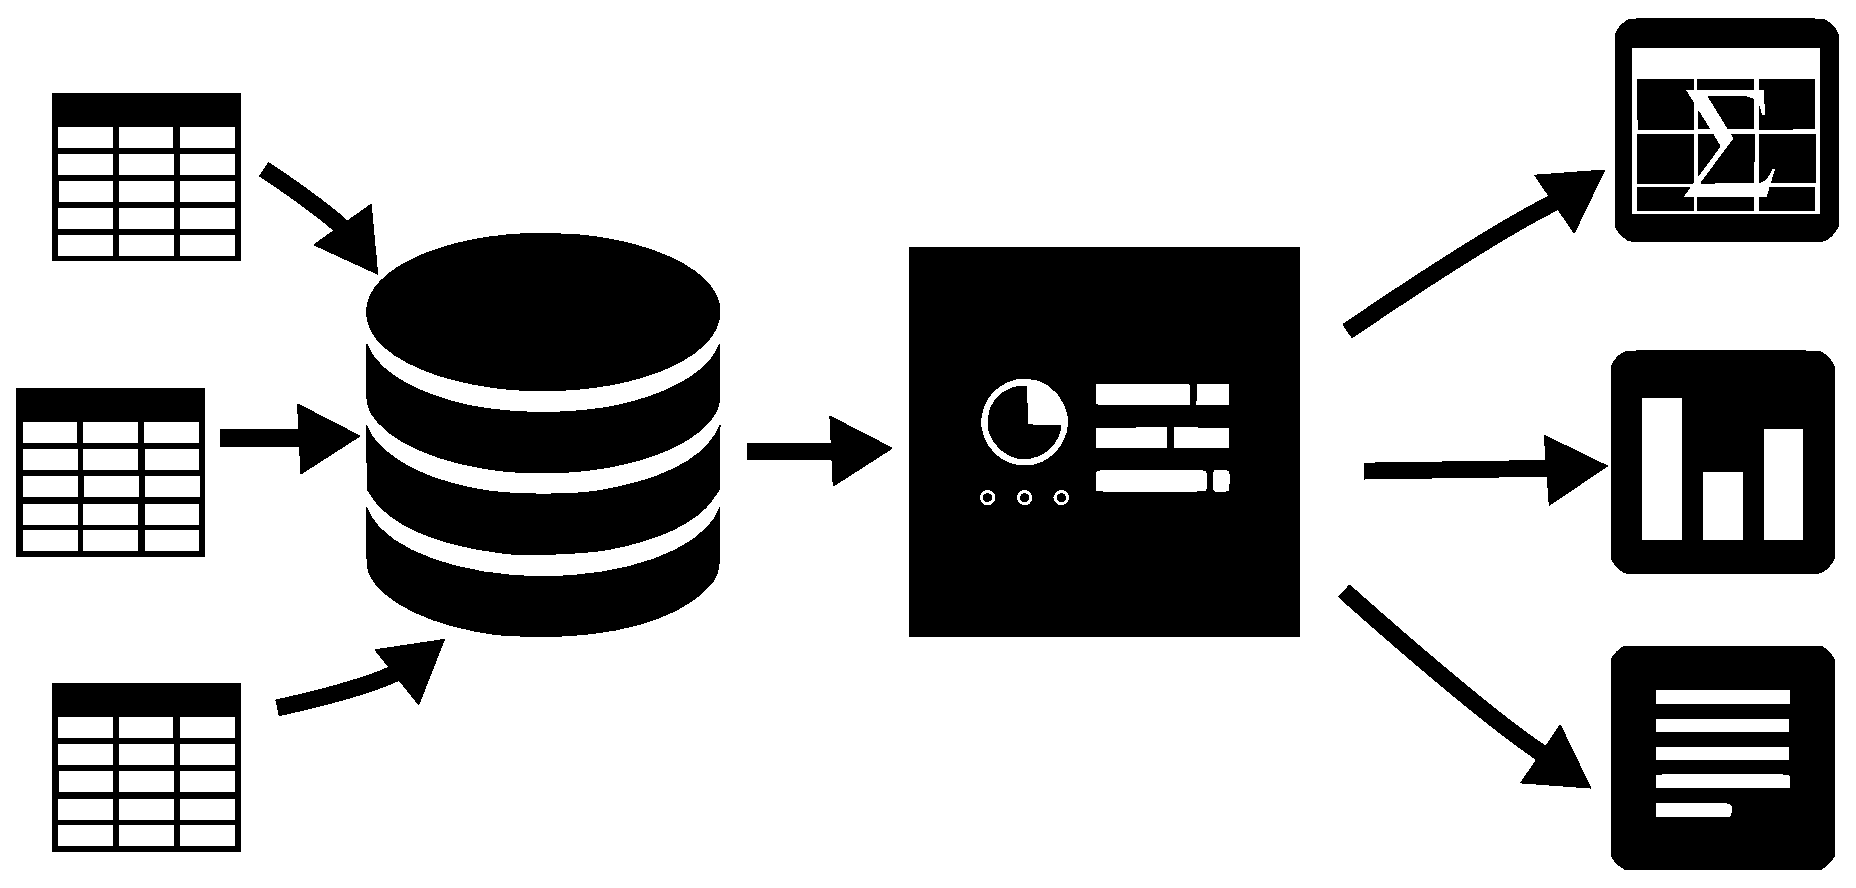
\includegraphics[width=\textwidth]{MVP3}}
 \end{overlayarea}
\end{frame}


\section{Fazit}
\subsection{Projektergebnis}
\begin{frame}{80\,\% Zeitersparnis}

\includegraphics[width=\textwidth]{Balken}
\end{frame}
\subsection{Lessons Learned}
\begin{frame}{}

\end{frame}

\end{document}

